\section{Problem 3}
\textit{Explain the connection – if possible- between table 2.6 and figure 2.58 in Mobile Antenna System Handbook on page 103-4 – the experimental results}\\

\begin{center}
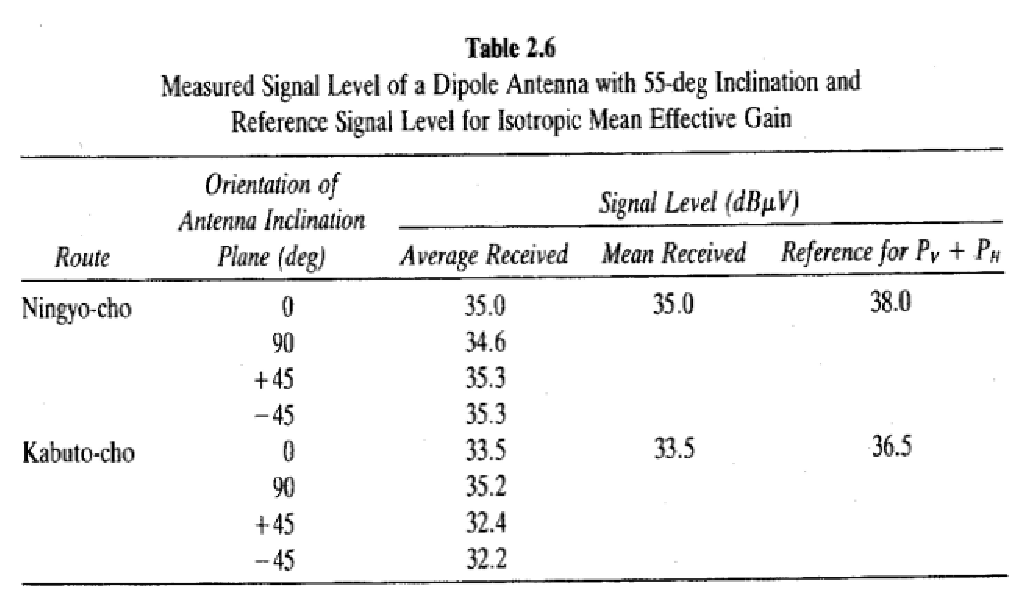
\includegraphics[scale=0.6]{figures/Tabel_2_6.eps}\\
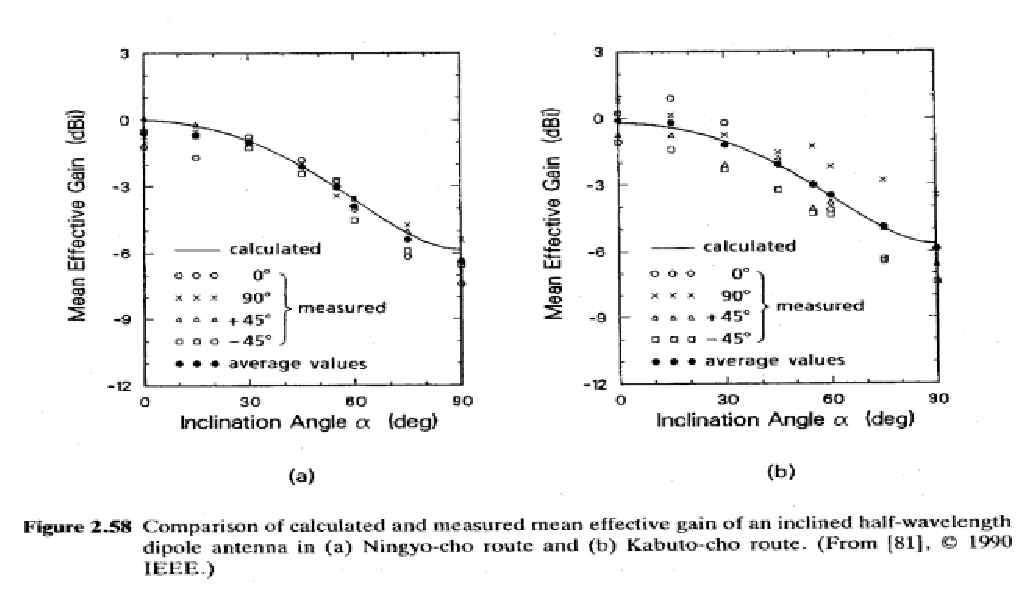
\includegraphics[scale=0.85]{figures/Figure_2_58.eps}
\end{center}

% I THINK IS BETTER NOT TO INCLUDE THE TABLE AND THE FIGURE AS LOCAL FIGURES SO IS EASIER FOR REFERRING AND MORE CLEAR TO UNDERSTAND

%Table 2.6 from the book is shown in \figref{fig:Tabel_2_6}:
%\fig[keepaspectratio=true,width=14cm]{Tabel_2_6.eps}{Table 2.6 from Mobile Antenna Systems Handbook }{fig:Tabel_2_6}
%Figure 2.58 from the book is shown in \figref{fig:Figure_2_58}:
%\fig[keepaspectratio=true,width=16cm]{Figure_2_58.eps}{Table 2.6 from Mobile Antenna Systems Handbook}{fig:Figure_2_58}

The figure 2.58 shows the results of the Mean Effective Gain of an antenna in two different cities in function of the inclination of the antenna dipole, and the orientation of the respective inclination plane (0,+45,-45,90).
 
On the other hand, the table 2.6 shows the numeric results of the received signal level of a dipole antenna in the same locations. The inclination of the antenna was fixed to 55° in order to get the reference for the $P_V + P_H$ (given that with this inclination the $P_{rec}$ is half of that independently from the XPR). Then it is measured the received signal while rotating the orientation of the antenna inclination plane. As the MEG is defined as:

\begin{flalign}
&& G_e &= \frac{P_{rec}}{P_V + P_H} &
\end{flalign}

Thus, it can be easily obtained the MEG for each orientation values by just subtracting the reference $P_V + P_H$ to each received power. Those MEG values correspond to the points showed in the figure 2.58 for $\alpha$=55.
